\documentclass[12pt]{article}
\usepackage{palatino}
\usepackage{a4wide}
\usepackage{hyperref}
\usepackage{graphicx}
\usepackage[parfill]{parskip}

\title{DigiApproval}
\author{Daniel Axtens, Andrew Donnellan, Benjamin Roberts}

\begin{document}
\maketitle

\section{Your summary of the Challenge}

A thriving, vibrant city should make it easy for citizens and small
businesses to run public events. At the same time, regulations and
permit systems are needed to make sure that events are run in a safe,
community-friendly and sustainable way.

Unfortunately, the proliferation of regulations and permits has made
running events into something more akin to navigating a maze. The point
of this challenge it to provide Canberrans with a simple, efficient way
to navigate the maze.

The goal of the challenge is to provide residents and businesses with a
clear, streamlined way to navigate the various approvals required. The
system should provide a central point of contact, so that, as far as
possible, a single public servant sees the process through from start to
finish and is able to help resolve problems as they come up. The system
should lay out the requirements clearly, providing tools like checklists
to ensure that applicants understand what is required of them and can
meet those requirements with a minimum of fuss.

\section{Your concept of how to address it}

Our solution is a web based \emph{workflow engine}, that provides
superior flexibility to directorates, a consistent user interface to
applicants, and utilises standardised components so it can be
constructed within 3 months and maintained cheaply and easily.
\newpage
\subsection{Underlying concept}

Our concept can be summarised as a flexible, web-based \emph{workflow
engine}.

\subsubsection{Introducing our characters}

\begin{itemize}
\itemsep1pt\parskip0pt\parsep0pt
\item
  An \emph{applicant} is someone trying to organise an event or apply
  for a permit.
\item
  A \emph{directorate} is the body that an applicant must work with to
  get one or more of the permits they require. Within a directorate,
  there are 3 roles:

  \begin{itemize}
  \item
    An \emph{administrator}, who sets up the application process in
    terms of workflows, as detailed bleow.
  \item
    An \emph{approver} works with an applicant to progress their
    application.
  \item
    A \emph{manager} is responsible for balancing the workload amongst
    approvers.
  \end{itemize}
\end{itemize}

\subsubsection{What is a workflow?}

A workflow is a tailored set of steps to achieve a particular outcome.
For example, applying for a permit to serve alcohol is a workflow, and
applying for a permit for traffic managment is a workflow. Workflows can
contain other workflows, and have optional steps, so the entire process
of organising an event could be one big workflow.

The concept of a workflow is sufficiently flexible to encompass the
range of steps and options in a practical approval process. 
\begin{itemize}
\item Workflows can contain steps that an applicant must take, and
  steps that an approving agency must take. These steps can contain a
  variety of steps: applicants steps can involve uploading documents,
  filling in forms, and so on; agency steps can include review,
  approval, etc.
\item Applicants and approvers are notified when the application
  changes from one state to another, for example by email.
\item Workflows do not need to be linear. For example, if an event
  management plan is insufficient, rather than rejecting the entire
  application, the applicant can be directed back to resubmitting the
  event management plan until it is satisfactory.
\item Workflows can be easily visualised as flow charts, so the status
  of an application is clear to the applicant and to the approving
  directorate at a glance.
\item Workflows can contain information about time limits: for example
  if required documentation is not sumbitted within the required time
  period, the workflow can automatically transition to an expired
  state.
\end{itemize}

A sample workflow demonstrating these features is shown below. This workflow
is a very simple sample of an approval process involving an event
management plan. Steps an applicant takes are blue, and steps approvers
take are green.

\begin{figure}[htbp]
\centering
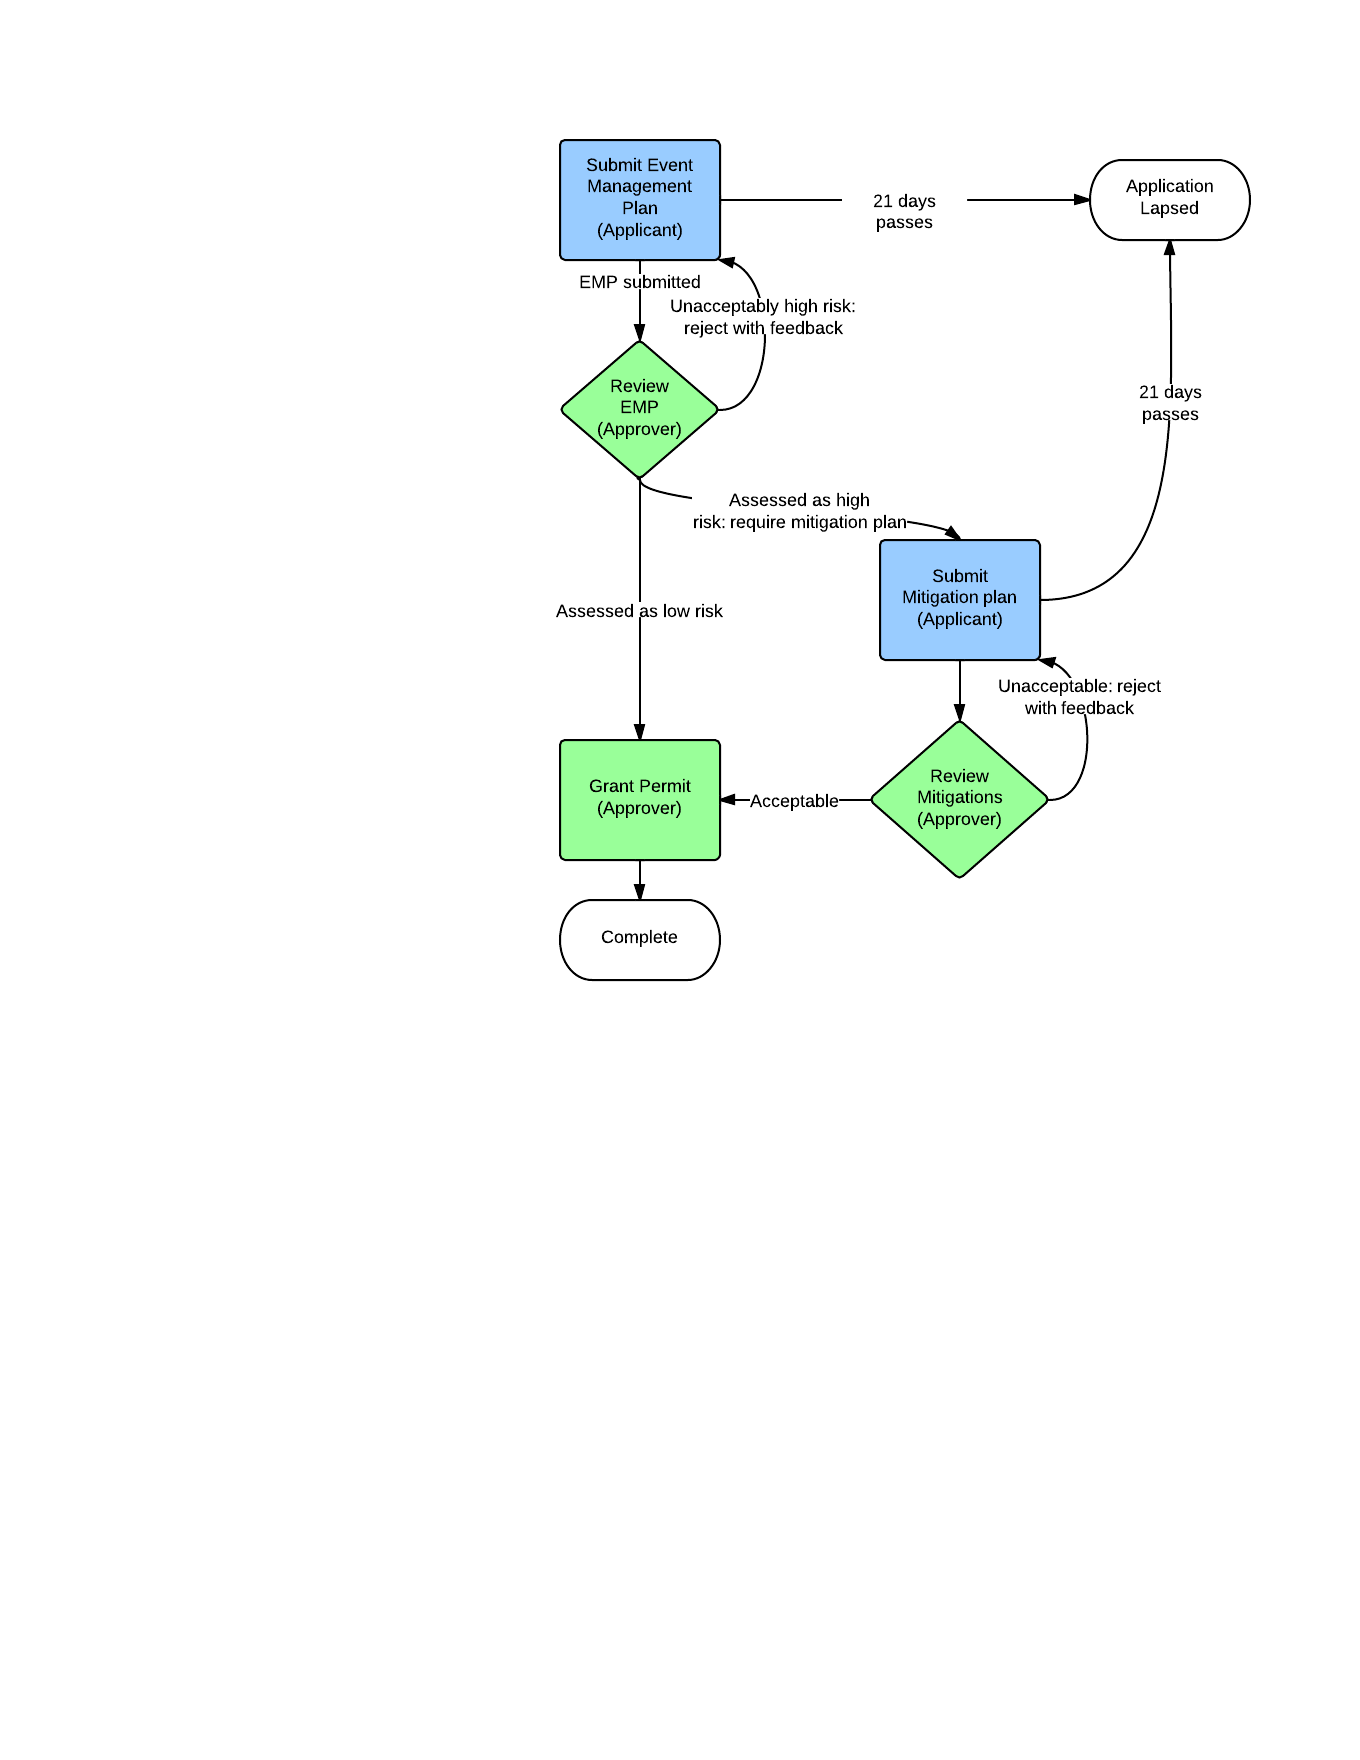
\includegraphics[width=0.82\textwidth]{./imgs/sample-workflow.png}
\caption{Sample workflow}
\end{figure}
\newpage
Workflows, as we have conceptualised them, have other benefits too: 
\begin{itemize}
\item Workflows can bring together all the relevant documentation in
  one place. A step that requires an applicant to upload a document
  can contain information about what the document is supposed to
  contain.  Steps that an approver must take can include information
  about how a document is to be reviewed, so as to ensure consistency
  amongst staff.  This information is not shown to applicants, so
  internal processes can be documented. 
\item Workflows can contain other workflows: for example a workflow
  for running an event could guide an applicant through the relevant
  approvals. Each of those approvals is its own workflow, so if an
  applicant knows they only need a specific permit, they can do that
  workflow individually. (This also means that individual directorates
  can update and improve the workflows for which they are responsible,
  without it breaking the overall process.)
\end{itemize}

\subsubsection{Setting up the system}

Before an applicant can use the system, an administrator must create
workflows. 
\begin{itemize}
\item A web interface will allow administrators to build fully
  functional workflows without requiring additional code to be
  written. The administrator will be able to specify the steps in the
  workflow, whether they are done by approvers or the applicant, and
  provide any information necessary for each step to be completed.
\item The web interface will be able to present the workflow as a flow
  chart, so that management within the directorate can easily verify
  that the web process matches up with legislative requirements and
  existing processes. 
\item The workflow will not be presented to the public until it is
  expressly made live.
\end{itemize}

\subsubsection{Using the system: applicant}

Before an applicant can begin a workflow, they must register as a user.

Once they register with their name and contact details, they will be
presented with a dashboard showing at a glance: 
\begin{itemize}
\item \textbf{Workflows that they can commence.} Once a workflow is
  commenced, the directorate is notified, and the application is
  assigned to an approver. 
\item \textbf{Any existing applications that they have begun}, and the
  stage those applications are at. Applicants can pull up the details
  of their applications and see the entire history in one place. They
  can then make sure that they have completed any steps necessary for
  them to complete.  The approver responsible for their application is
  notified whenever the applicant completes a step. 
\item \textbf{A link to contact the approver assigned to help them
    progress their workflow}. 
\item \textbf{A link to access completed applications}, should they
  need to re-download any documents/approvals.
\end{itemize}
A very loose concept of what this might look like is shown below.

\begin{figure}[htbp]
\centering
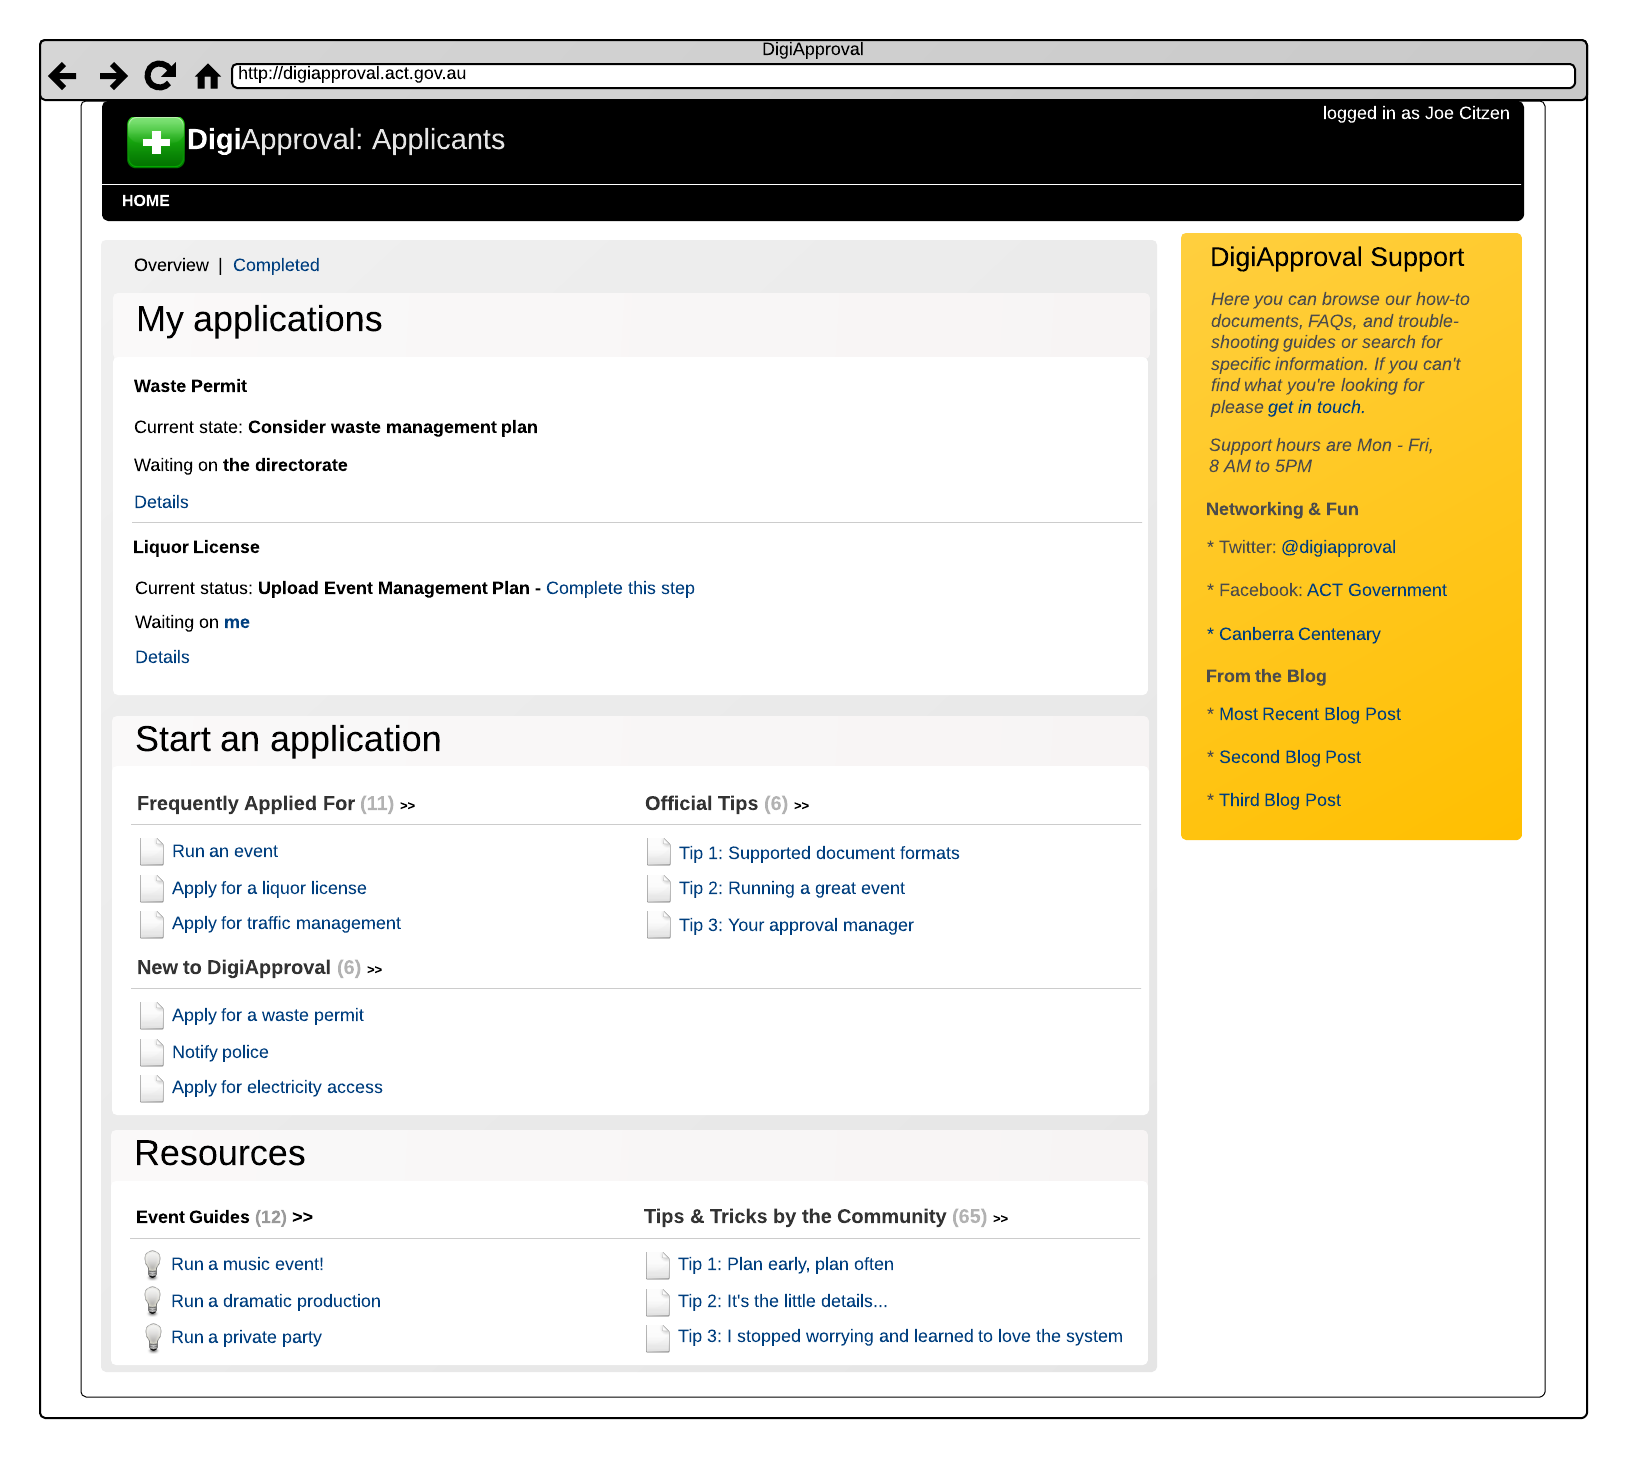
\includegraphics[width=0.98\textwidth]{./imgs/user-wireframe.png}
\caption{Potential user wireframe}
\end{figure}
\newpage
\subsubsection{Using the system: approvers}

The workflow system streamlines the job of those tasked with improving
applications and makes it easy for them to provide excellent service.

When an approver logs in, they can see at a glance: 
\begin{itemize}
\item The applications for which they are responsible.
\item The status of those applications: are they waiting on the
  applicant, or are they ``in my court''?
\end{itemize}

Approvers can then pull up an application for which they are
responsible, see its entire history in one place, and take any steps
necessary to progress it. The applicant is notified whenever the
approver completes a step.

A very loose concept of what this might look like is shown below.

\begin{figure}[htbp]
  \centering
  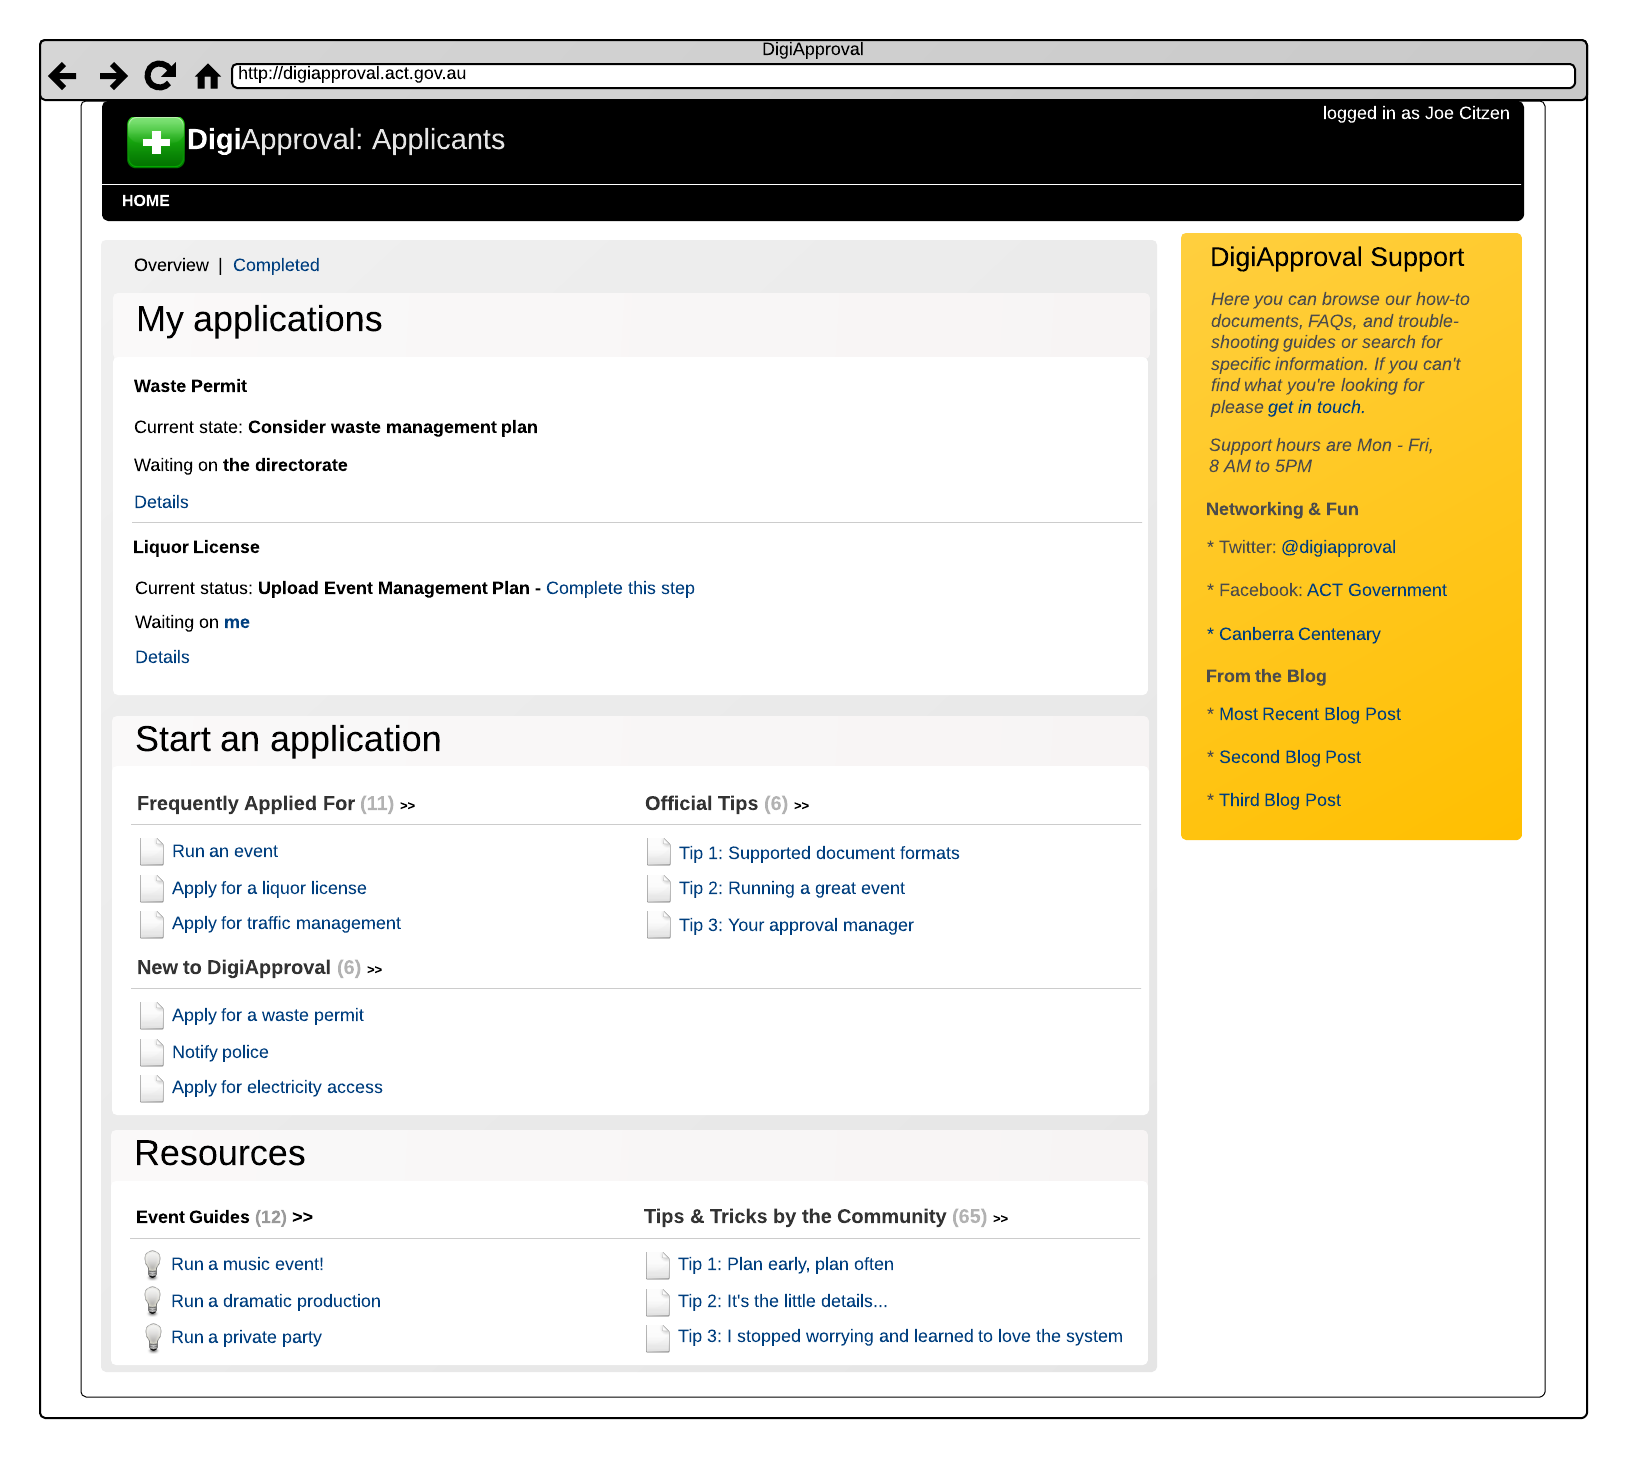
\includegraphics[width=0.98\textwidth]{./imgs/approver-wireframe.png}
\caption{Potential approver wireframe}
\end{figure}

\subsubsection{Using the system: managers}

Managers are responsible for allocating approvers to handle various
requests. A manager assigns a workflow that has just commenced to an
approver, and is able to re-allocate in-progress workflows if needed.
(For example, if an approver is ill or leaves the directorate.)

\subsubsection{Summary of concept}

The key advantages of our approach are: 

\begin{itemize}
\item Flexiblity: changes to procedures not require programmer
  intervention 
\item Consistency: Applicants deal with a consistent approver, while
  the directorate retains the flexibility to change approvers if the
  circumstances require it.
\item Central repository for information and state: all parties
  involved can see the progress at a glance, who has to take the next
  step.
\end{itemize}

\subsection{Implementation}

We intend to implent the system in \href{http://django.org}{Django}, a
well known web framework for the Python programming language. Django is
used on sites that deal with millions of hits, so it is known to be able
to scale. It is also has a large community of users: if we are hit by a
bus, it will be easy to find Django developers to keep the system
running.

The implementation will focus on scalability, security and portability.

\subsubsection{Scalibility}

The solution has been designed from the ground up for scalability, by
decoupling and disaggregating functions into layers that are known to be
scalable.

As the diagram on the next page shows, our solution can be decomposed into a web layer,
an application layer, a set of asynchronous workers and a storage layer
(file store and database).

\begin{figure}[htbp]
\centering
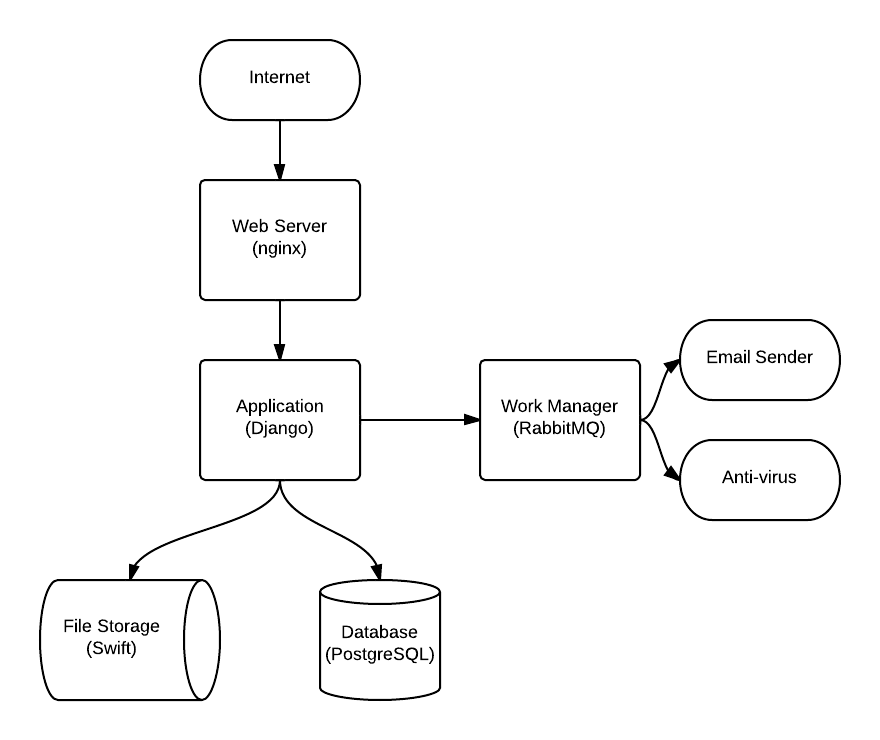
\includegraphics[width=0.98\textwidth]{./imgs/tech-overview.png}
\caption{Application architecture}
\end{figure}
\newpage
Each of these layers is horizontally scalable: if heavy usage of the
web layer is detected, additional web server can be added without
requring any changes to the application code. Similarly, if the
database is slow, the database layer can be scaled without requiring
the application code to be changed. An example of a scaled up
configuration is shown below.

\begin{figure}[htbp]
\centering
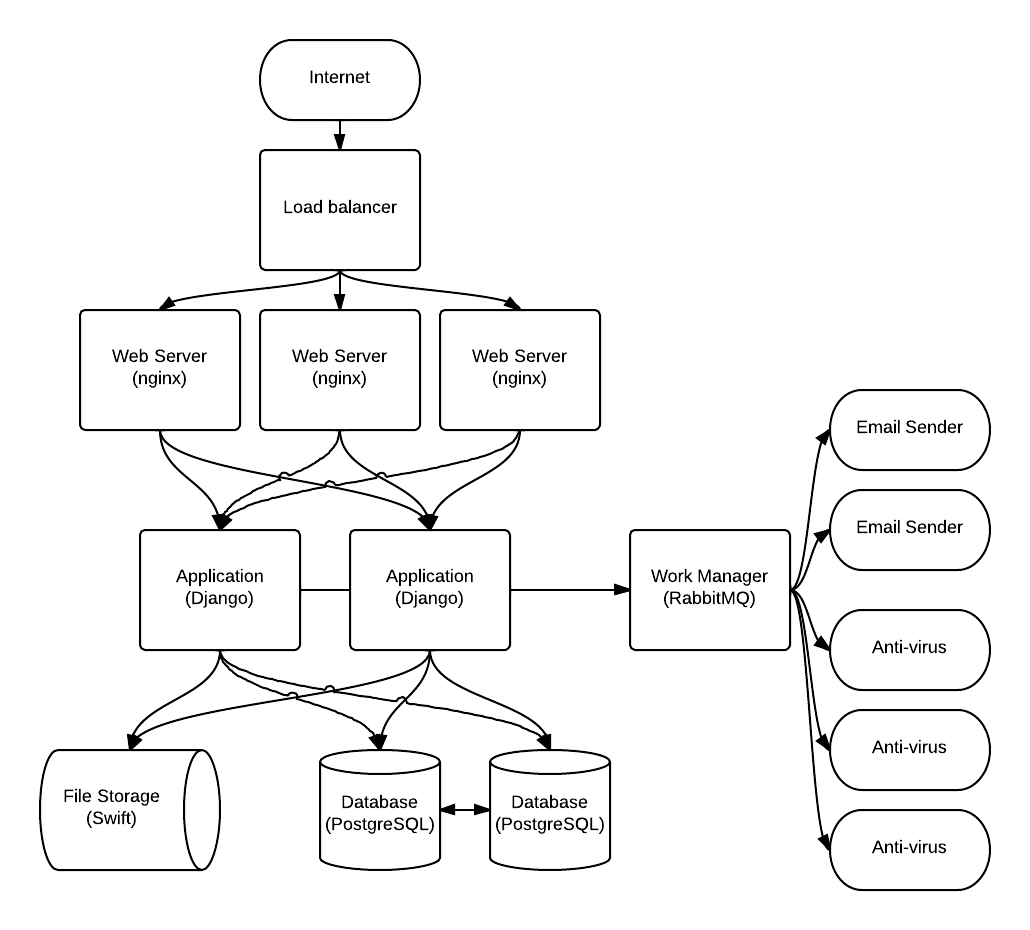
\includegraphics[width=0.98\textwidth]{./imgs/tech-scaling.png}
\caption{Example of a way to scale the application}
\end{figure}

Each layer can be scaled to suit demand, allowing scaling to address the
bottleneck without adding unnecessary infrastructure. Similarly, the
whole system can be scaled down: the entire system could concievably be
run on a single server if demand is not too great.

\subsubsection{Security}

Our system is designed to be able to solidly \emph{authenticate} users,
determine what those user are \emph{authorised} to do, ensure the
\emph{integrity} of their actions and the system as a whole, while
maintaining \emph{confidentially} of applicant and directorate
information, using industry best practices.

We will deploy SSL at the front end to ensure applicant passwords and
information is encrypted while in transit. We will be implementing as
much functionality as possible through standard libraries, reducing the
scope for security flaws and error on our part.

We will also be taking a proactive approach to security wherever
possible. For example, a major source of security flaws arise from not
verifying user input. Our system will make sure that we that user input
is valid, make sure that uploaded documents are of the expected format
and are free from known viruses, and so on, \emph{before} they are
presented to approvers.

\subsubsection{Portability}

We will be developing our system on Amazon Web Services (AWS), however
our system will not depend on any feature of the AWS infrastructure.
This provides flexibility in regards to the systems final hosting
environment; whether that be AWS or not. For example if control of data
is a concern, the system could be moved to government systems without
needing to rewrite sections of the codebase.

We will be ensuring this by using proven, industry-standard, open-source
technologies throughout.

Our current proposed stack is:
\begin{itemize}
\item Our web layer will be implemented with
  \href{http://nginx.org/en}{nginx}.
\item As discussed, our application layer will be implemented with
  Django.
\item Our worker layer will be implented using
  \href{http://rabbitmq.com}{RabbitMQ}. Having a worker model allows
  us to perform time-consuming tasks such as scanning for viruses or
  sending emails without making our user interface
  non-responsive. 
\item Our database layer will be implemented with
  \href{http://postgresql.org}{PostgreSQL}. 
\item Our file storage layer will be implemented using
  \href{http://swift.openstack.org}{OpenStack Swift}.
\end{itemize}

If necessary, we may substitute other standard, proven, open-source
technologies.

\section{Your proposed project milestones}

We propose the following milestones:

\begin{itemize}
\item
  By the end of week 1: Infrastructure set up, technology stack working.
\item
  By the end of week 4: Static (manually coded) workflows work.
\item
  During week 9/10: Dynamic (user entered) workflows can be created and
  work.
\end{itemize}

We will then use the time until the end of week 12 to polish the user
interface and catch up on any missed milestones. Providing this ``buffer
time'' means we are better equiped to deal with any unexpected issues
that develop.

\section{The critical dependencies}

\subsection{Key Assumptions}

\begin{itemize}
\item
  Directorate procedures are, or can be, reduced to a workflow. Given
  that they are bureaucratic processes, this should be possible.
\end{itemize}

\subsection{Key Requirements}

\begin{itemize}
\item
  Directorate involvement to help define a proof-of-concept workflow.
\item
  Directorate feedback to inform and refine the prototype as it
  develops.
\item
  Some costs, as detailed below.
\end{itemize}

\section{Likely costs}

Our main cost will be hosting. To ensure we design in a scalable way, we
will be using a number of instances on AWS. This prevents us from
accidentally making assumptions that will not hold true if the system is
scaled up. Our estimate is for 6 AWS t1.micro instances for 3 months,
for an estimated \$75/month, or \$225 for the duration of the bake-off.

We will also have some one-off costs associated with an SSL certificate.
This will cost around \$75.

Our total estimated costs are \$300.

\section{Your full solution assessment}

The full details for our proof-of-concept are listed above.

Assuming our proof-of-concept is successful, the following major steps
would be required to deploy it publically:
\begin{itemize}
\item \textbf{The services of a skilled graphics designer}. We
  have a range of coding and user-experience skills, but we lack good
  graphics skills. A skilled graphics designer would be needed to make
  things aesthetically appealing and consistent with the rest of the
  visual identity across the ACT government. 
\item \textbf{A further period of development}. Our prototype will
  inevitably have some rough edges. It will need an extra couple of
  months of full-time work to bring it up to a deployable standard,
  especially with regards to:
  \begin{itemize}
  \item accessibility (e.g.~to WCAG 2.0 standard)
  \item load-testing 
  \item fault tolerance and testing 
  \item documentation
  \end{itemize}
\item \textbf{Deployment on government servers.}
\item \textbf{Training of users within departments.} This is probably
  going to be the most time-consuming aspect of a final
  deployment. Users will need to be trained to work with the
  application, create work-flows, and IT staff will need to be trained
  to support the system.
\end{itemize}

\newpage
\section{Your eligibility}

I, Daniel Axtens, declare:
\begin{itemize}
\item I am an ACT resident and a tertiary student at The
  Australian National University (u5376292) \item There are no
  conflicts of interest arising if I am involved in implementing the
  challenge.
\end{itemize}


I, Andrew Donnellan, declare:
\begin{itemize}
\item I am an ACT resident and a tertiary student at The
  Australian National University (u4837946) \item There are no
  conflicts of interest arising if I am involved in implementing the
  challenge.
\end{itemize}


I, Benjamin Roberts, declare:
\begin{itemize}
\item I am an ACT resident and a tertiary student at The
  Australian National University (u5350335) \item There are no
  conflicts of interest arising if I am involved in implementing the
  challenge.
\end{itemize}

\end{document}